This path-sensitive reachability-bound algorithm
is performed on basis of an \emph{Abstract Transition Graph} for the program $c$.
An \emph{Abstract Transition Graph}, $\absG(c) =(\absV(c), \absE(c))$ for a program $c$ is composed of
a vertex set $\absV(c)$ and an edge set $\absE(c)$.
%
% \\
% Every 
% vertex $l \in \absV(c)$ corresponds to a program point $l$, which is a unique
% label of a command in this program.
% $\absV(c)$ is the set of $c$'s all program points,
% \\
% \subsection{Edges}
% \label{sec:abs_prog-edge}
%   In the first step, we generate the \textbf{constraint}
%   for the expression in each program command,
%   which is used as the annotation of each edge.
%   \\
% The second step generates two sets for each command, which are \textbf{Initial and Continuation Execution State}. 
%   The initial execution state contains the
%   program points where this command {starts} to execute, 
%   and the continuation execution state contains both the constraint of this command
%   and the continuation program points after the execution of this command.
%   \\ 
%   In the third step, we compute the \textbf{Abstract Event} and generate the set of edges for the program.
%   Each edge composed of an initial and a continuation execution state.
%

\begin{defn}[Symbolic Constant, Symbolic Expression]
  \label{def:symbolic_expr}
The universe of the \emph{symbolic constant} is denoted by $\scvardom \subseteq \mathbb{N} \cup \vardom \cup \{\infty \}$, in which a symbolic constant can be a natural number, $\infty$, or a program's input variable.
 The \emph{symbolic expression} of a program $\scexpr(c) \subseteq \mathcal{A}$ is the set of all the arithmetic expressions over $\mathbb{N} \cup \inpvar(c) \cup \{\infty \}$ for the program $c$.
\end{defn}

\begin{defn}[Difference Constraints]
 The difference constraints $DC(\vardom  \cup \scvardom)$ is the set of all the inequality of
form $x' \leq y + v$ or $x' \leq v$ where $x, y \in \vardom $ and $v \in \scvardom$.
An inequality $x' \leq y + v$ describes that the value of $x$ in the current state is
at most the value of $y$ in the previous state plus the symbolic constant $v$, and $x' \leq v$ describes that the value of $x$ in the current state is
at most $v$.
\end{defn}

\begin{defn}[Constraints]
A constraints $dc \in \dcdom^{\top} = DC(\vardom  \cup \scvardom) \cup \booldom\cup \{\top\}$  can be either a
difference constraint $d \in DC(\vardom  \cup \scvardom)$, a boolean expression $\bexpr \in \booldom$
or $\top$ denotes always true.
\end{defn}

When the constraint that shows up as an edge annotation is a difference constrain, $l \xrightarrow{x' \leq y + v} l'$,
% Then $x'$ 
it denotes that
the value of variable $x$
after executing the command at $l$ is at most
% and the right-hand side describes 
the value of variable $y$ plus $v$ before the execution,
and $l \xrightarrow{x' \leq v} l'$ respectively denotes
% value of variable $x$
% after executing the command at $l$ is 
$x$ has at most
% and the right-hand side describes 
the value of the symbolic constant $v$.
%  before the execution.
For example in Figure~\ref{fig:relatedNestedWhileOdd-overview}(b), constraint $i' \leq i - 1$ on the edge $7 \xrightarrow{i' \leq i - 1} 1$
describes the execution of
 the command at line $7$, 
$\clabel{\assign{i}{i - 1}}^{7}$. 

% For every expression in each of the label command, it is computed in three steps via program abstraction method adopted from the Section~6 in~\cite{SinnZV17}. 

The boolean constraint, $\bexpr$ on an edge $l \xrightarrow{b} l'$ describes
that after evaluating the guard with label $l$,
$\bexpr$ holds and the command with label $l$ will execute right after.
For example, the boolean constraint $i \leq 0 $ on the edge $1 \xrightarrow{i \leq 0} \lex$, 
represents the negation of the testing guard $\clabel{i > 0}^1$
in the $\ewhile$ command, and $i \leq 0$ must hold in order to perform this transition from program point $1$ to
the program exit. 
We also have $\top$, which is preserved for $\eskip$ command or the commands that don't interfere any guard variable.

\begin{defn}[Abstract Transition Graph]
  \label{def:abs_cfg}
  The \emph{abstract transition graph} of a program $c$ is $\absG(c) \triangleq (\absV(c), \absE(c))$, where
  $\absV(c) \triangleq \lvar(c)\cup\{\lex\}$
  and 
  % $\absE(c) \triangleq \{(l_1, dc, l_2) | (l_1, dc, l_2) \in \absflow(c)\}$,
  % and
  % .
  each edge $(l, dc, l') \in \absE(c)$ is an abstract transition
between two program points $l, l'$ if and only if
the command with label $l'$ can execute right after the execution of the command with label $l$.
% if and only if there is a control flow between two program points.
The constraint $dc \in \dcdom$ on each edge is generated from the command with label $l$, which describes the abstract execution of this command.
\end{defn}
Again in Figure~\ref{fig:relatedNestedWhileOdd-overview}(b),
the edge $(0 \xrightarrow{i' \leq n} 1)$ on the top tells us the command 
$\clabel{\assign{i}{n}}^0$ is executed with a continuation point $1$, and the while loop with header at location $1$ , $\ewhile \clabel{i > 0}^1 \edo \{\ldots\}$ will be executed right after.

\begin{defn}[Path]
  \label{def:abs_cfgpath} 
  A path on $\absG(c)$ is a sequence, $ l_0 \xrightarrow{dc_0} l_1 \xrightarrow{dc_1} \ldots $ with
  \begin{itemize}
  \item the vertices sequence $(l_0, \ldots)$, where $l_i \in \absV(c)$ for every $i = 0, 1, \ldots$ and
  %
  \item the edge sequence $(e_0, \ldots)$, where $e_i = (l_{i}, dc_i, l_{i + 1}) \in \absE(c)$ for every $i = 0, 1, \ldots$.
  \end{itemize}
  A path is cyclic, if it has the same start- and end-point. A path is simple, if it does not visit a location twice except for start- and end-location. We use $\paths(\absG(c))$ to denote the set of all the paths on $\absG(c)$,
  and $\pathl(p)$ to represent the list of program points corresponding to the vertices sequence of this path $p \in \paths(\absG(c))$,
  where $\pathl : \paths(\absG(c)) \to \mathcal{P}{(\ldom)}$.
  \end{defn}
  For example, $1 \to 2 \to 3 \to 4 \to 5 \to 4$ in Figure~\ref{fig:relatedNestedWhileOdd-overview}(b) is a \emph{path}, but it is not simple (the program points $4$ is visited twice). The path $4 \to 5 \to 4$ is both cyclic and simple.

  % \\
  % \subsection{Abstract Transition Graph of The Walk through Example}
  % \label{sec:abs_prog_example}
  % 
% \paragraph*{Walk Through Example}
% %\begin{example}
 % [The Running Example with Nested Loop in One Path]
%  \label{ex:relatedNestedWhileOdd-overview}
{ \small
% \vspace{-0.2cm}
\begin{figure}
\centering
\begin{subfigure}{.4\textwidth}
\begin{centering}
{\small
$
\begin{array}{l}
  \kw{nestedOdd}(n, m) \triangleq \\
  \clabel{ \assign{i}{n} }^{0} ; \\
      L_1: \ewhile ~ \clabel{i > 0}^{1} ~ \edo ~ \\
      \quad \big(
        \eif(\clabel{i \% 2 \neq 0 }^{2},
        \clabel{\assign{k}{i - m}}^{3};\\
        \quad L_4: \ewhile ~ \clabel{k > 0}^{4} \edo \\
        \quad ( \clabel{\assign{k}{k - 1}}^{5} );\\
        \quad \clabel{\assign{i}{k + m}}^{6};
        \clabel{\assign{i}{i - 1}}^{7}, \\
        \quad \clabel{\assign{i}{i - 3}}^{8})
        \big)
  \end{array}
$
}
\vspace{-0.3cm}
\caption{}
\end{centering}
\end{subfigure}
\begin{subfigure}{.52\textwidth}
\begin{centering}
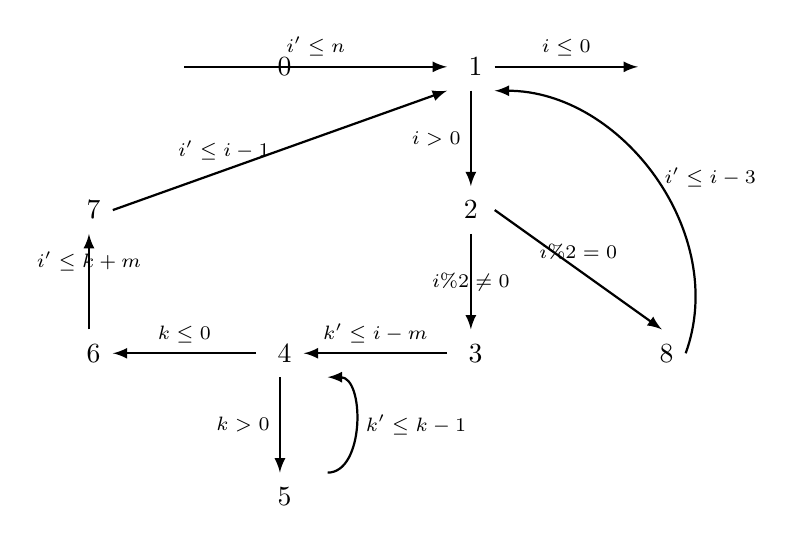
\begin{tikzpicture}[scale=\textwidth/20cm,samples=200]
\draw[] (-4, 10) circle (0pt) node{{ $0$}};
\draw[] (0, 10) circle (0pt) node{{ $1$}};
\draw[] (0, 7) circle (0pt) node{\textbf{$2$}};
\draw[] (0, 4) circle (0pt) node{{ $3$}};
\draw[] (-4, 4) circle (0pt) node{{ $4$}};
\draw[] (-8, 4) circle (0pt) node{{ $6$}};
\draw[] (-4, 1) circle (0pt) node{{ $5$}};
\draw[] (4, 4) circle (0pt) node{{ $8$}};
\draw[] (-8, 7) circle (0pt) node{{ $7$}};
% Counter Variables
\draw[] (4.5, 10) circle (0pt) node {\textbf{$\lex$}};
% \draw[] (6, 4) circle (0pt) node {{ $ex$}};
%
% Control Flow Edges:
\draw[ thick, -latex] (-6, 10)    -- node [above]{\scriptsize $i' \leq n$}(-0.5, 10);
\draw[ thick, -latex] (0, 9.5)    -- node [left] {\scriptsize $i > 0$} (0, 7.5) ;
\draw[ thick, -latex] (0.5, 7)    -- node [above] {\scriptsize $ i \% 2 = 0 $}  (4, 4.5);
\draw[ thick, -latex] (4.5, 4)    to  [out=70,in=0]   node [right] {\scriptsize $i' \leq i - 3$ }(0.5, 9.5);
\draw[ thick, -latex]  (0, 6.5)   -- node  {\scriptsize $i \% 2 \neq 0$}  (0, 4.5) ;
\draw[ thick, -latex]  (-0.5, 4)  -- node [above] {\scriptsize $k' \leq i - m$ }  (-3.5, 4) ;
\draw[ thick, -latex]  (-4.5, 4)  -- node [above] {\scriptsize $k \leq 0$ }  (-7.5, 4);
\draw[ thick, -latex] (0.5, 10)   -- node [above] {\scriptsize $i \leq 0$}  (3.5, 10);
\draw[ thick, -latex] (-4, 3.5)   -- node [left] {\scriptsize $k > 0$}  (-4, 1.5);
\draw[ thick, -latex] (-3, 1.5)   to  [out=0,in=0] node [right] {\scriptsize $k' \leq k- 1$}  (-3, 3.5);
\draw[ thick, -latex] (-8, 4.5)   --  node [above] {\scriptsize $i' \leq k + m$ }(-8, 6.5);
\draw[ thick, -latex] (-7.5, 7)  --  node [left] {\scriptsize $i' \leq i - 1$ }(-0.5, 9.5);
% \draw[ thick, -latex] (6, 6.5)  -- node [right] {$\top$} (6, 4.5) ;
\end{tikzpicture}
\vspace{-0.5cm}
\caption{}
\end{centering}
\end{subfigure}
\begin{subfigure}{.9\textwidth}    
\begin{centering}
{\small
$\tpath_0 = (0 \to 1)$
\quad
$\tpath_1 = (1 \to 2 \to 3 \to 4)$
\quad
$\tpath_2 = (4 \to 6 \to 7 \to 1)$
\quad
$\tpath_3 = (4 \to 5 \to 4)$
\quad
$\tpath_4 = (1 \to 2 \to 8 \to 1)$
\quad
$\tpath_5 = (1 \to \lex)$
}
\vspace{-0.3cm}
\caption{}
\end{centering}
\end{subfigure}
% \vspace{-0.5cm}
\begin{subfigure}{.8\textwidth}    
  \begin{centering}
  $
  \tpath_0 ; \rpchoose{ 1: \rprepeat(\tpath_1; 4:\rprepeat(\tpath_3); \tpath_2; \tpath_4), 
  1: \rprepeat(\tpath_4; \tpath_1; 4:\rprepeat(\tpath_3); \tpath_2) }; \tpath_5
  $
  % \vspace{-0.5cm}
  \caption{}
  \end{centering}
  \end{subfigure}
\caption{
(a) Running example: program with a loop with two  paths and a nested loop in one of them,
(b) the corresponding \emph{abstract transition graph}, $\absG(\kw{nestedOdd}(n, m))$,
(c) all the simple transition paths on this program,
(d) the refined program.}
% \vspace{-0.75cm}      
\label{fig:relatedNestedWhileOdd-overview}
\end{figure}
}
%  \footnotetext{In the transition path, $(l_0 \to \cdots \to l_n)$, the constraints are omitted for concise.}
%
%  \end{example}    

% Our running example in Figure~\ref{fig:relatedNestedWhileOdd-overview}(a) has two paths loop with different reachability-bounds on the control
% locations in different paths.
% Its abstract control flow graph is shown in Figure~\ref{fig:relatedNestedWhileOdd-overview}(b).
% The edge $(0 \xrightarrow{i' \leq n} 1)$ on the top tells us the command 
% $\clabel{\assign{i}{n}}^0$ is executed with a continuation point $1$, and the
% command $\ewhile \clabel{i > 0}^1 \edo \{\ldots\}$ will be executed next.
% The annotation $i' \leq n$ is a difference constraint 
% computed by $\absexpr$ over
% the expression $n$ in the assignment command $\assign{i}{n}$.
% It represents that the value of $i$ is less than or equal to value of $n$ after the
% execution of $\clabel{\assign{i}{n}}^0$ and before evaluating the guard $\clabel{i > 0}^1$.
% Another example constraint $i' \leq i - 1$ on the edge $7 \xrightarrow{i' \leq i - 1} 1$
% describes the execution of
%  the command at line $7$, 
% $\clabel{\assign{i}{i - 1}}^{7}$. 
% The $i'$ on the left side of $i' \leq i - 1$ represents the value of $i$ after the assignment operation,
% and the right-hand side $i$ stores the value before the assignment.
% The boolean constraint $i \leq 0 $ on the edge $1 \xrightarrow{i \leq 0} \lex$, 
% represents the negation of the testing guard $\clabel{i > 0}^1$
% in the $\ewhile$ command.
% $1 \xrightarrow{i \leq 0} \lex$ denotes that $i \leq 0$ must hold in order to perform this transition from program point $1$ to
% the program exit. 
% \paragraph{Constraint Computation}
% In this step, we first show how to compute the constraints for expressions in a program $c$,
% by a program abstraction method adopted from the
% algorithm in Section 6 in~\cite{SinnZV17}.
% \\
% Given a program $c$,
% every arithmetic expression in an assignment command with label $l$,
% or boolean expression in the guard of a $\eif$ or $\ewhile$ command with label $l$
% is transformed into a constraint.
% \\
% This constraint describes the abstract execution of the assignment command with label $l$,
% or abstract evaluation of the boolean expression in the guard with label $l$.

% \highlight{Notations / Formal Definitions:}
% \begin{itemize}
% \item Operator: $\absexpr : \mathcal{A} \cup \booldom \to DC(\vardom  \cup \scvardom)\cup \booldom \cup \{\top\}$
% %
% \item Constraints $\dcdom^{\top}: DC(\vardom  \cup \scvardom) \cup \booldom\cup \{\top\}$  contains:
% %
% \begin{itemize}
% \item The difference constraints $DC(\vardom  \cup \scvardom)$ is the set of all the inequality of
% form $x' \leq y + v$ or $x' \leq v$ where $x \in \vardom $, 
% $y \in \vardom$ and $v \in \scvardom$.
% \\
% The \emph{Symbolic Constant} can be a natural number, $\infty$, or a program's input variable, We use $\scvardom \subseteq \mathbb{N} \cup \vardom \cup \{\infty \}$ to denote the universe of all \emph{Symbolic Constant},
% which is the set of all natural numbers with $\infty$ and programs' input variables.
% \\
% An inequality $x' \leq y + v$ describes that the value of $x$ in the current state is
% at most the value of $y$ in the previous state plus the symbolic constant $v$.
% An inequality $x' \leq v$ describes that the value of $x$ in the current state is
% at most the value $v$.
% When a difference constrain shows up as an edge annotation, $l \xrightarrow{x' \leq y + v} l'$,
% % Then $x'$ 
% it denotes that
% the value of variable $x$
% after executing the command at $l$ is at most
% % and the right-hand side describes 
% the value of variable $y$ plus $v$ before the execution,
% and $l \xrightarrow{x' \leq v} l'$ respectively denotes value of variable $x$
% after executing the command at $l$ is at most
% % and the right-hand side describes 
% the value of the symbolic constant $v$ before the execution.
% For every expression in each of the label command, it is computed in three steps via program abstraction method adopted from the Section~6 in~\cite{SinnZV17}. 
% %
% \item The Boolean Expressions $b$ from the set $\booldom$.
% $b$ on an edge $l \xrightarrow{b} l'$ describes
% that after evaluating the guard with label $l$,
% $b$ holds and the command with label $l$ will execute right after.
% %
% \item The top constraint, $\top$ denotes true. It is preserved for $\eskip$ command,
% or commands that don't interfere any guard variable.
% \end{itemize}
% \end{itemize}

% \highlight{Computation Steps:}

% \begin{defn}[Symbolic Constant, Symbolic Expression of a Program($\scexpr(c)$)]
%   \label{def:symbolic_expr}
%   $\scexpr(c)$ is the set of all the arithmetic expressions over $\mathbb{N} \cup \inpvar(c) \cup \{\infty \}$ for a given program $c$.
% % \end{defn}

% \begin{defn}[Constraint Computation]
%   \label{def:constraint_compute}
%   For a program $c$, a boolean expression $\bexpr$ in the guard of a $\eif$ or $\ewhile$ command
%   or an expression $\expr$ and a variable $x$
%   in an assignment command $\assign{x}{\expr}$,
%   the constraint $\absexpr(\bexpr, \_, c )$ or $\absexpr(x - v, x, c)$ is computed as follows.
%   \begin{enumerate}
%   \item Compute the symbolic constant set of program $c$, $\scvar(c)$ of program $c$ as follows.
%   \[
%     \scvar(c) = \mathbb{N} \cup \inpvar(c) \cup \{\infty \} \subseteq \scvardom
%   \]
%   \item Initialize 
%   $\grdvar(c) = \{\}$ as the set of the variable used in the expression of every while or if guard in the program $c$.
%   \item Then we compute  $\absexpr(\bexpr, \_, c )$ or $\absexpr(x - v, x, c)$.
%   \[
%     \begin{array}{ll} 
%       \absexpr(x - v, x, c)  = x' \leq x - v  & x \in \grdvar(c)\land v \in \scvar(c) \\
%       \absexpr(y + v, x, c)  = x' \leq y + v  & x, y \in \grdvar(c)\land v \in \scvar(c)\\
%       \absexpr(v, x, c)  = x' \leq v  & x \in \grdvar(c)\land v \in \scvar(c) \\
%       \absexpr(y + v, x, c)  = x' \leq y + v, \grdvar(c) = \grdvar(c) \cup \{y\} 
%       & x \in \grdvar(c)\land y \notin \grdvar(c) \land v \in \scvar(c)  \\
%       \absexpr(\bexpr, \_, c) = \bexpr, \grdvar(c) = \grdvar(c) \cup FV(\bexpr) & \bexpr \in \scvar(c) \\
%       \absexpr(\expr, x, c) = \top &  {o.w.} \\
%     \end{array}
%     \]
%   \end{enumerate}
%    $\absexpr(\expr, x, c)$ and $\grdvar(c)$ are iteratively updating until stabilized over every guard and assignment command in $c$. In the following part of the paper, we use $\absexpr(\expr, x, c)$
%    to denote the stabilized computation result.
%   \end{defn}
% %
% In the case 4, if a variable $x$, belonging to the set 
%   $\grdvar(c)$ is updated by a variable $y$, which isn't in this set, 
%   we add $y$ into the set $\grdvar(c)$ and repeat 
%   above procedure  until $\grdvar(c)$ and $\absexpr(\expr, x, c)$ is stabilized. 
%   \\
% Specifically 
% we handle a 
% normalized expression, $x > 0$
% in guards of if and while loop headers, and 
% the guard variable $x$ only increase, decrease or reset by 
% simple arithmetic expression (mainly multiplication, division, minus and plus (able to extend to max and min)). 
% The guard variable $x$ is generalized into the \emph{norm} when the guard 
% in if or while has the form $\expr > 0$ with an expression $\expr$, and $\grdvar$ is the set of norms.
% Then in the last clause in Definition~\ref{def:constraint_compute}, i.e., $\absexpr(\expr, x, c)$,
% we will check if $\expr$ is a norm or contains norms, and extend the $\grdvar(c)= \grdvar(c)\cup \{\expr\}$ if neither.
% The constraint computation over the \emph{norm} follows the computation steps 1, 2 and 3 in Section 6.1 in paper~\cite{SinnZV17}. 
% %
% \paragraph{Abstract Initial and Continuation Execution State Computation}
% This step computes two sets for each command. 
% The initial execution state is a set that contains the
% program points before executing this command, which is computed by the standard initial state generation method from control flow analysis.
% The continuation execution state is a set
% that contains the constraint of this command and the program points after the execution of this command.
% This set is enriched 
% from the standard control flow analysis.

% %
% \begin{itemize}
%   \item The \emph{initial execution state}, $\absinit(c) \in \ldom$
%   for a command $c$.
%   $\absinit(c)$ is a unique program label corresponds to the command before executing this command. 
% \\
% Given a program $c$, its abstract initial execution state, $\absinit(c)$ is computed as follows,
% %
% \[
%   \begin{array}{ll}
%     \absinit(\clabel{\assign{x}{\expr}}{}^l)  & = l  \\
%     \absinit(\clabel{\eskip}^{l})  & = l \\
%     \absinit(\eif (\clabel{\bexpr}^l, c_t, c_f))  & = l \\
%     \absinit(\ewhile \clabel{\bexpr}^l \edo (c_w))  & = l \\
%     \absinit(c_1 ; c_2)  & = \absinit(c_1) \\
%  \end{array}
%  \]
% %
% %
% \item The \emph{continuation execution state}, $\absfinal(c)$ of program $c$, 
% $\absfinal(c) \in \mathcal{P}(\ldom \times \dcdom^{\top})$
% is a set of pairs, $(l, dc)$ with a
% program point (i.e., a label), $l$ as the first component and a constraint, 
% $dc$ as the second component.
% The program point $l$ corresponds to the labeled command after the execution of $c$,
% and the constraint $dc$ in this pair is computed by $\absexpr$ for the expression in $c$.
% \\
% Given a program $c$, its continuation execution state, $\absfinal(c)$ is computed as follows,
%  \[
%   \begin{array}{ll}
%     \absfinal(\clabel{\assign{x}{\expr}}{}^l)  & = \{(l, \absexpr(\expr, x, c))\}  \\
%      \absfinal(\clabel{\eskip}^{l})  
%      & = \{(l, \top)\} \\
%      \absfinal(\eif (\clabel{\bexpr}^l, c_t, c_f))  & = \absfinal(c_t) \cup \absfinal(c_f) \\
%      \absfinal(\ewhile \clabel{\bexpr}^l \edo (c_w))  & = \{(l, \absexpr(\bexpr, \top, c_w))\} \\
%      \absfinal(c_1 ; c_2)  & =  \absfinal(c_2) \\
%  \end{array}
%  \]
%  %
% \end{itemize}
%  \paragraph{Abstract Event Computation} Each abstract event is an edge between two vertices in the abstract transition graph.
%  It is generated by computing the initial and continuation execution state interactively and recursively for a program $c$.
 
%  \highlight{Notations and Formal Definitions:}
%  \begin{itemize}
%   \item \emph{Abstract Event}: 
%   $\absevent \in $
%   $\ldom \times \dcdom^{\top} \times \ldom$
%   \item \emph{Abstract Trace}, $\absflow(c)$ of a program $c$: $\absflow(c) \in \mathcal{P}( \ldom \times \dcdom^{\top} \times \ldom )$
%  \end{itemize}
%  \begin{defn}[Abstract Event]
%    \label{def:abs_event}
%    Abstract Event: 
%    $\absevent \in $
%    $\ldom \times \dcdom^{\top} \times \ldom$
%    is a 
%    triple where the first and third components are labels,
%    second component is a constraint from $\dcdom^{\top}$.
%    \end{defn}
%    In an abstract event $(l, dc, l')$ of a program $c$, 
%    the first label $l \in \ldom$ corresponds to the \emph{initial execution point} $\absinit(c)$ of $c$, and 
%    the second label $l' \in \ldom$ with the constraint $dc \in \dcdom^{\top}$ correspond to an abstract continuation execution state of $c$.
% We abuse the notation $\mathcal{P}(\absevent)$ for the power set of all abstract events.

% \highlight{Computation Steps:}
% \\
% The set of the abstract events $\absflow(c)$ for a program $c$
% is computed as follows in Definition~\ref{def:absevent_compute}.
%  %
%  \begin{defn}[Abstract Trace Computation]
%  \label{def:absevent_compute}
%  The \emph{abstract trace}, $\absflow(c) \in \mathcal{P}( \ldom \times \dcdom^{\top} \times \ldom )$ of a program $c$  is computed as follows.

%  We first append a $\eskip$ command with 
% the label $\lex$, i.e., $\clabel{\eskip}^{{\lex}}$ at the end of the program $c$, and construct 
% the program $c' = c;\clabel{\eskip}^{{\lex}}$.
% Then, we compute the $\absflow(c) = \absflow'(c')$ for $c'$ as follows,
%  %
%  {
%  \[
%    \begin{array}{ll}
%       \absflow'(\clabel{\assign{x}{\expr}}{}^l)  & = \emptyset  \\
%       \absflow'([\eskip]^{l})  & = \emptyset \\
%       \absflow'(\eif (\clabel{\bexpr}^l, c_t, c_f))  & =  \absflow'(c_t) \cup \absflow'(c_f)
%         \\ & \quad 
%         \cup \{(l, \absexpr(\bexpr, \top, c),  \absinit(c_t) ) ,  (l, \absexpr(\neg\bexpr, \top, c), \absinit(c_f)) \} \\
%        \absflow'(\ewhile \clabel{\bexpr}^l \edo (c_w))  & =  \absflow'(c_w) \cup \{(l, \absexpr(\bexpr, \top, c), \absinit(c_w)) \} 
%        \\ & \quad 
%        \cup \{(l', dc, l)| (l', dc) \in \absfinal(c_w) \} \\
%        \absflow'(c_1 ; c_2)  & = \absflow'(c_1) \cup  \absflow'(c_2) 
%        \\ & \quad 
%        \cup \{ (l, dc, \absinit(c_2)) | (l, dc) \in \absfinal(c_1) \} \\
%    \end{array}
%    \]
%    }
%   \end{defn}
%   Notice $\absflow'([x := \expr]^{l})$ and $\absflow'([\eskip]^{l})$ are both empty set. 
%    For every event $\event$ with label $l$ in an execution trace $\trace$ of program $c$, 
%    there is an abstract event in program's abstract execution trace of form $(l, \_, \_)$.  
%    We also show the soundness of the \emph{abstract event computation} as Theorem~\ref{lem:abscfg_sound} below with proof in Appendix~\ref{apdx:abs_sound}.
% \begin{lem}[Soundness of the Abstract Trace Computation]
% \label{lem:abscfg_sound}
% For every program $c$ and
% a finite execution trace $\trace \in \ftdom$ which is generated w.r.t.
% an initial trace  $\trace_0 \in \ftdom_0(c)$,
% there is an abstract event $\absevent = (l, \_, \_) \in \absflow(c)$ 
% for every event $\event \in \trace$ having the same label $l$, i.e., $\event = (\_, l, \_)$.
% %
% \[
% \begin{array}{l}
%   \forall c, c' \in \cdom, \trace_0 \in \ftdom_0(c), \trace \in \ftdom ,  \event = (\_, l, \_) \in \eventset \st
%   \big(
%     \config{{c}, \trace_0} \to^{*} \config{c', \trace_0 \tracecat \trace} 
%   % \lor 
%   % \config{{c}, \trace_0} \uparrow^{\infty} \trace_0 \tracecat \trace 
%   \big)
%   \land \event \in \trace 
%   \\
%   \qquad \implies \exists \absevent = (l, \_, \_) \in (\ldom\times \dcdom^{\top} \times \ldom) \st 
%   \absevent \in \absflow(c)
% \end{array}
% \]
% \end{lem}
% If $l$ is the label of an assignment command in a program $c$,
% then there is a unique abstract event in the program's abstract events set
% $\absevent \in \absflow(c)$ of form $(l, \_, \_)$. This uniqueness property is formally below as Lemma~\ref{lem:abscfg_unique} below
% and proved in Appendix~\ref{apdx:abs_sound}.
% \begin{lem}[Uniqueness of the Abstract Events]
% \label{lem:abscfg_unique}
% For every program $c$ and
% a finite execution trace $\trace \in \ftdom$ which is generated w.r.t.
% an initial trace $\trace_0 \in \ftdom_0(c)$,
% there is a unique abstract event $\absevent = (l, \_, \_) \in \absflow(c)$ 
% for every assignment event $\event \in \eventset^{\asn}$ in the
% execution trace having the label $l$, i.e., $\event = (\_, l, \_)$ and $\event \in \trace$.
% %
% \[
%   \begin{array}{l}
%   \forall c \in \cdom, \trace_0 \in \ftdom_0(c), \trace \in \ftdom ,  \event = (\_, l, \_) \in \eventset^{\asn} \st
%   \big(
%     \config{{c}, \trace_0} \to^{*} \config{c', \trace_0 \tracecat \trace} 
%   % \lor 
%   % \config{{c}, \trace_0} \uparrow^{\infty} \trace_0 \tracecat \trace 
%   \big)
%   \land \event \in \trace 
%   \\
%   \qquad \implies \exists ! \absevent = (l, \_, \_) \in (\ldom\times \dcdom^{\top} \times \ldom) \st 
%   \absevent \in \absflow(c)
%   \end{array}
% \]
% \end{lem}
% %
% \paragraph{Edge Construction}
% The edge for $c$'s abstract transition graph is constructed simply by computing the program's abstract events set, $\absflow(c)$ as follows,
%   \[
%     \absE(c) = \{(l_1, dc, l_2) | (l_1, dc, l_2) \in \absflow(c)\}
%   \]
% For each edge $(l, dc, l') \in \absE(c)$, $dc$ describes either an abstract execution of the assignment command with label $l$,
% or the evaluation of the guard with label $l$.
% %
% \subsection{Abstract Transition Graph Construction} 
% With the vertices $\absV(c)$ and edges $\absE(c)$ ready, we construct the abstract transition graph, formally in
% Definition~\ref{def:abs_cfg}.
%
% \begin{defn}[Abstract Transition Graph]
% \label{def:abs_cfg}
% Given a program $c$, 
% its \emph{abstract transition graph} $\absG(c) \triangleq (\absV(c), \absE(c))$ where
% $\absE(c) \triangleq \{(l_1, dc, l_2) | (l_1, dc, l_2) \in \absflow(c)\}$,
% and
% $\absV(c) \triangleq \lvar(c)\cup\{\lex\}$.

% A path on $\absG(c)$ is a sequence, $ l_0 \xrightarrow{dc_0} l_1 \xrightarrow{dc_1} \ldots $ with
% \begin{itemize}
% \item the vertices sequence $(l_0, \ldots)$, where $l_i \in \absV(c)$ for every $i = 0, 1, \ldots$ and
% %
% \item the edge sequence $(e_0, \ldots)$, where $e_i = (l_{i}, dc_i, l_{i + 1}) \in \absE(c)$ for every $i = 0, 1, \ldots$.
% \end{itemize}
% A path is cyclic, if it has the same start- and end-point. A path is simple, if it does not visit a location twice except for start- and end-location. We use $\paths(\absG(c))$ to denote the set of all the paths on $\absG(c)$,
% and $\pathl(p)$ to represent the list of program points corresponding to the vertices sequence of this path $p \in \paths(\absG(c))$,
% where $\pathl : \paths(\absG(c)) \to \mathcal{P}{(\ldom)}$.
% \end{defn}
% % \\
% \subsection{Abstract Transition Graph of The Walk through Example}
% \label{sec:abs_prog_example}
% % 
% %\begin{example}
 % [The Running Example with Nested Loop in One Path]
%  \label{ex:relatedNestedWhileOdd-overview}
{ \small
% \vspace{-0.2cm}
\begin{figure}
\centering
\begin{subfigure}{.4\textwidth}
\begin{centering}
{\small
$
\begin{array}{l}
  \kw{nestedOdd}(n, m) \triangleq \\
  \clabel{ \assign{i}{n} }^{0} ; \\
      L_1: \ewhile ~ \clabel{i > 0}^{1} ~ \edo ~ \\
      \quad \big(
        \eif(\clabel{i \% 2 \neq 0 }^{2},
        \clabel{\assign{k}{i - m}}^{3};\\
        \quad L_4: \ewhile ~ \clabel{k > 0}^{4} \edo \\
        \quad ( \clabel{\assign{k}{k - 1}}^{5} );\\
        \quad \clabel{\assign{i}{k + m}}^{6};
        \clabel{\assign{i}{i - 1}}^{7}, \\
        \quad \clabel{\assign{i}{i - 3}}^{8})
        \big)
  \end{array}
$
}
\vspace{-0.3cm}
\caption{}
\end{centering}
\end{subfigure}
\begin{subfigure}{.52\textwidth}
\begin{centering}
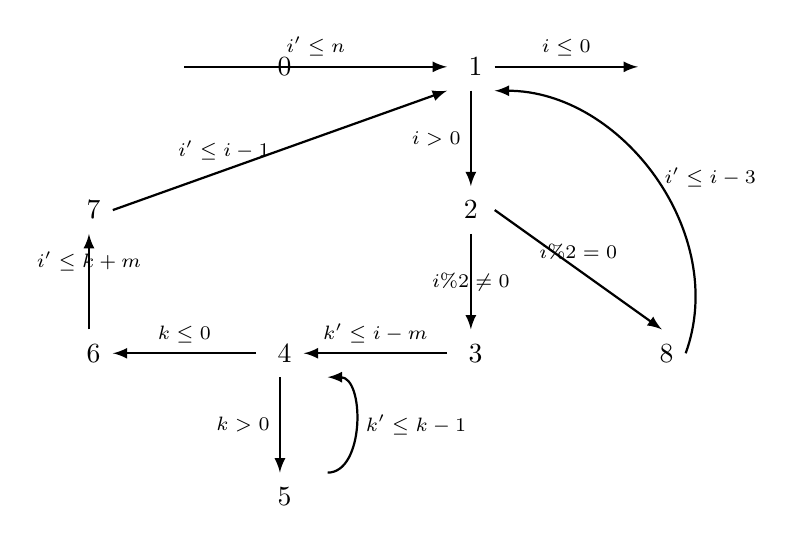
\begin{tikzpicture}[scale=\textwidth/20cm,samples=200]
\draw[] (-4, 10) circle (0pt) node{{ $0$}};
\draw[] (0, 10) circle (0pt) node{{ $1$}};
\draw[] (0, 7) circle (0pt) node{\textbf{$2$}};
\draw[] (0, 4) circle (0pt) node{{ $3$}};
\draw[] (-4, 4) circle (0pt) node{{ $4$}};
\draw[] (-8, 4) circle (0pt) node{{ $6$}};
\draw[] (-4, 1) circle (0pt) node{{ $5$}};
\draw[] (4, 4) circle (0pt) node{{ $8$}};
\draw[] (-8, 7) circle (0pt) node{{ $7$}};
% Counter Variables
\draw[] (4.5, 10) circle (0pt) node {\textbf{$\lex$}};
% \draw[] (6, 4) circle (0pt) node {{ $ex$}};
%
% Control Flow Edges:
\draw[ thick, -latex] (-6, 10)    -- node [above]{\scriptsize $i' \leq n$}(-0.5, 10);
\draw[ thick, -latex] (0, 9.5)    -- node [left] {\scriptsize $i > 0$} (0, 7.5) ;
\draw[ thick, -latex] (0.5, 7)    -- node [above] {\scriptsize $ i \% 2 = 0 $}  (4, 4.5);
\draw[ thick, -latex] (4.5, 4)    to  [out=70,in=0]   node [right] {\scriptsize $i' \leq i - 3$ }(0.5, 9.5);
\draw[ thick, -latex]  (0, 6.5)   -- node  {\scriptsize $i \% 2 \neq 0$}  (0, 4.5) ;
\draw[ thick, -latex]  (-0.5, 4)  -- node [above] {\scriptsize $k' \leq i - m$ }  (-3.5, 4) ;
\draw[ thick, -latex]  (-4.5, 4)  -- node [above] {\scriptsize $k \leq 0$ }  (-7.5, 4);
\draw[ thick, -latex] (0.5, 10)   -- node [above] {\scriptsize $i \leq 0$}  (3.5, 10);
\draw[ thick, -latex] (-4, 3.5)   -- node [left] {\scriptsize $k > 0$}  (-4, 1.5);
\draw[ thick, -latex] (-3, 1.5)   to  [out=0,in=0] node [right] {\scriptsize $k' \leq k- 1$}  (-3, 3.5);
\draw[ thick, -latex] (-8, 4.5)   --  node [above] {\scriptsize $i' \leq k + m$ }(-8, 6.5);
\draw[ thick, -latex] (-7.5, 7)  --  node [left] {\scriptsize $i' \leq i - 1$ }(-0.5, 9.5);
% \draw[ thick, -latex] (6, 6.5)  -- node [right] {$\top$} (6, 4.5) ;
\end{tikzpicture}
\vspace{-0.5cm}
\caption{}
\end{centering}
\end{subfigure}
\begin{subfigure}{.9\textwidth}    
\begin{centering}
{\small
$\tpath_0 = (0 \to 1)$
\quad
$\tpath_1 = (1 \to 2 \to 3 \to 4)$
\quad
$\tpath_2 = (4 \to 6 \to 7 \to 1)$
\quad
$\tpath_3 = (4 \to 5 \to 4)$
\quad
$\tpath_4 = (1 \to 2 \to 8 \to 1)$
\quad
$\tpath_5 = (1 \to \lex)$
}
\vspace{-0.3cm}
\caption{}
\end{centering}
\end{subfigure}
% \vspace{-0.5cm}
\begin{subfigure}{.8\textwidth}    
  \begin{centering}
  $
  \tpath_0 ; \rpchoose{ 1: \rprepeat(\tpath_1; 4:\rprepeat(\tpath_3); \tpath_2; \tpath_4), 
  1: \rprepeat(\tpath_4; \tpath_1; 4:\rprepeat(\tpath_3); \tpath_2) }; \tpath_5
  $
  % \vspace{-0.5cm}
  \caption{}
  \end{centering}
  \end{subfigure}
\caption{
(a) Running example: program with a loop with two  paths and a nested loop in one of them,
(b) the corresponding \emph{abstract transition graph}, $\absG(\kw{nestedOdd}(n, m))$,
(c) all the simple transition paths on this program,
(d) the refined program.}
% \vspace{-0.75cm}      
\label{fig:relatedNestedWhileOdd-overview}
\end{figure}
}
%  \footnotetext{In the transition path, $(l_0 \to \cdots \to l_n)$, the constraints are omitted for concise.}
%
%  \end{example}    
